\documentclass[11pt]{article}
\usepackage{textcomp,geometry,graphicx,verbatim}
\usepackage{fancyhdr}
\usepackage{amsmath,amssymb,enumerate}
\pagestyle{fancy}
\def\Name{Manohar Jois}
\def\Homework{5} % Homework number - make sure to change for every homework!
\def\Session{Fall 2014}

% Extra commands
\let\origleft\left
\let\origright\right
\renewcommand{\left}{\mathopen{}\mathclose\bgroup\origleft}
\renewcommand{\right}{\aftergroup\egroup\origright}
\newcommand{\N}{\mathbb{N}}
\newcommand{\Z}{\mathbb{Z}}
\newcommand{\R}{\mathbb{R}}
\newcommand{\Q}{\mathbb{Q}}
\newcommand{\C}{\mathbb{C}}
\newcommand{\p}[1]{\left(#1\right)}
\renewcommand{\gcd}[1]{\text{gcd}\p{#1}}
\renewcommand{\deg}[1]{\text{deg}\p{#1}}
\renewcommand{\log}[1]{\text{log}\p{#1}}
\renewcommand{\ln}[1]{\text{ln}\p{#1}}
\newcommand{\logb}[2]{\text{log}_{#1}\p{#2}}
\newcommand{\BigOh}[1]{O\p{#1}}
\newcommand{\BigOmega}[1]{\Omega\p{#1}}
\newcommand{\BigTheta}[1]{\Theta\p{#1}}

\title{CS164\ \Session\  --- Answers to Homework \Homework}
\author{\Name}
\lhead{CS164\ \Session\  Homework \Homework\ Problem \theproblemnumber,\ \Name}

\begin{document}
\maketitle
\newcounter{problemnumber}
\setcounter{problemnumber}{0}

\section*{Exercise 1}
\stepcounter{problemnumber}
\begin{enumerate}[(a)]
\item The given grammar cannot generate the given parse tree because on the left side there are nodes that represent the rule (N $\to$ '-' N) which is not a grammar production.
\item $\phantom{A}$ \\
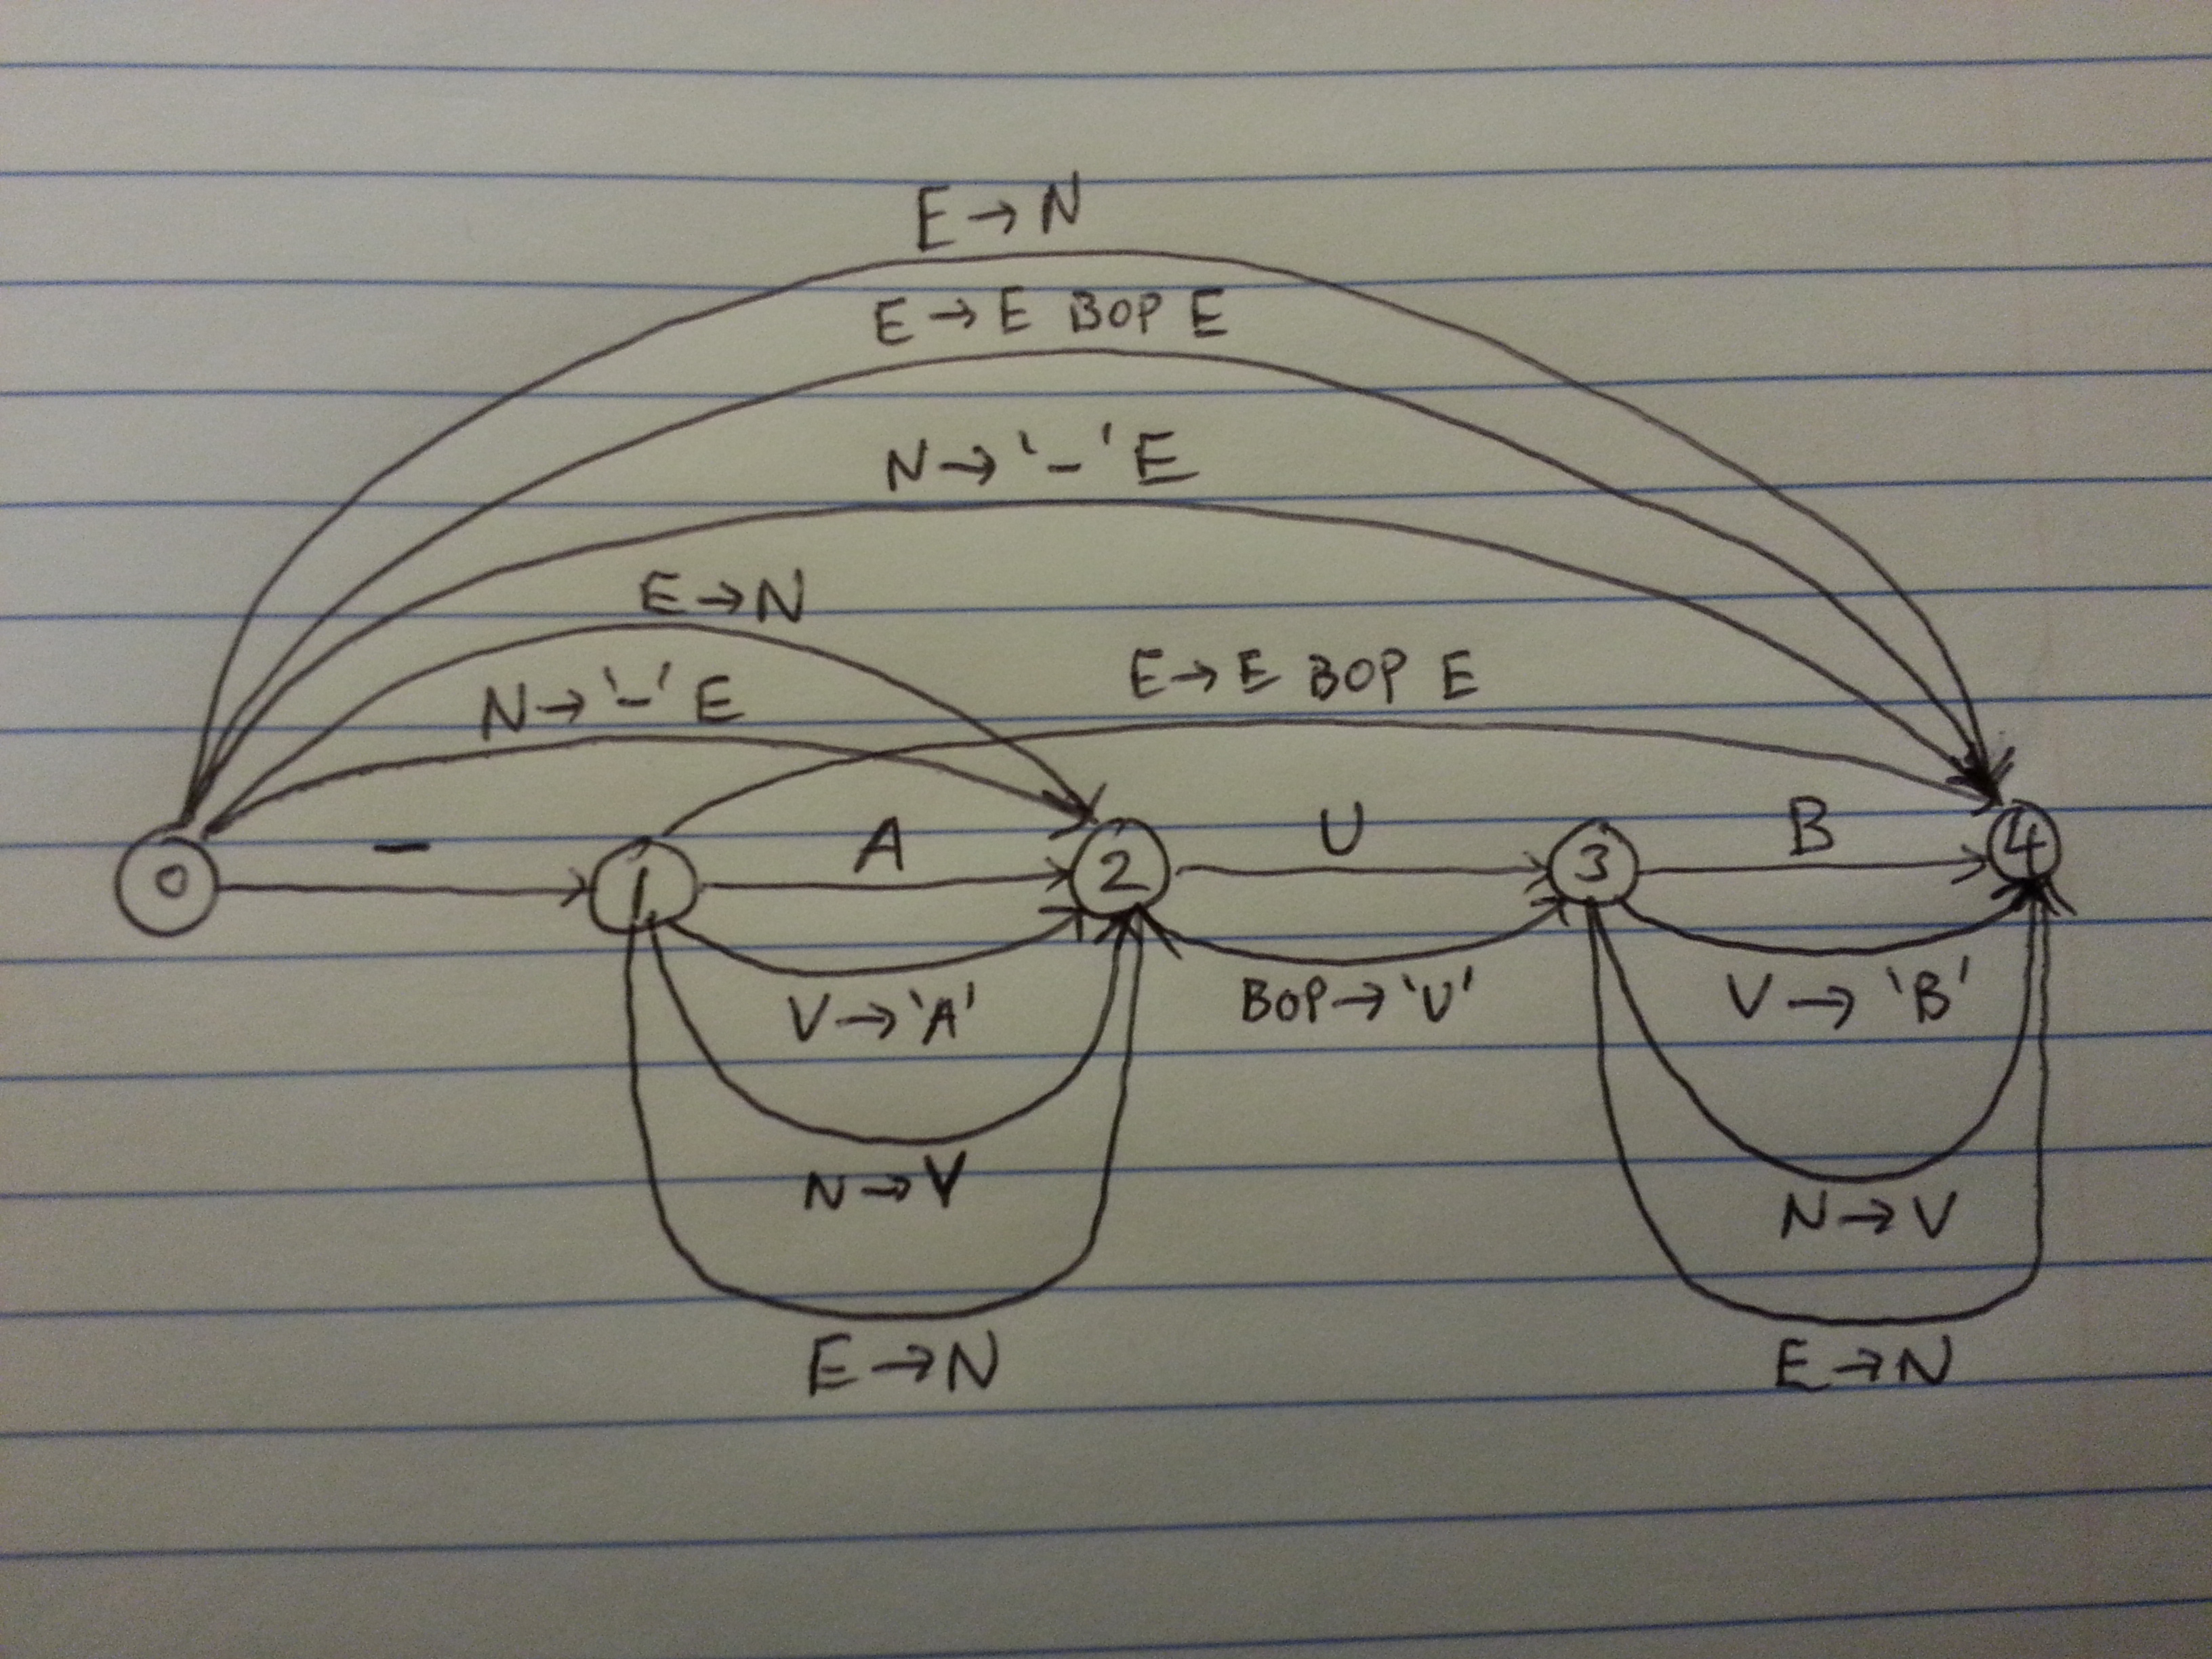
\includegraphics[scale=0.125]{earley}
\item The productions (E $\to$ E BOP E) and (BOP $\to$ '$\cup$' $|$ '-') lead to ambiguity in the final edge of the input $A \cup B - C$. When constructing the Earley graph, in both cases the final edge will be of the production (E $\to$ E BOP E), so it will be impossible to distinguish which edge is the correct parse based on binary operator precedence.
\item The parser doesn't correctly define the precedence for binary set difference. This can be fixed by moving the directive \texttt{\%left '-'} above the first directive. This works because the mechanism that gives unary complement higher precedence than binary operators is implemented by the \texttt{\%dprec} directives.
\item \begin{tabular}{ccl}
E1 & $\to$  & E1 '$-$' E2\\
   & $\mid$ & E2\\
E2 & $\to$  & E2 '$\cup$' N\\
   & $\mid$ & E2 '$\cap$' N\\
   & $\mid$ & N\\
N  & $\to$  & '$($' E1 '$)$'\\
   & $\mid$ & '$-$' N\\
   & $\mid$ & V\\
V  & $\to$  & 'A' $\mid$ 'B' $\mid$ 'C' $\mid$ 'D'
\end{tabular}
\end{enumerate}

\end{document}